%!TEX root = ../main.tex
\chapter{Surface Second-Harmonic Generation Yield}
\minitoc

In this chapter I walk the reader through the considerations for developing the
three layer (3-layer) model for the SSHG yield, and then derive explicit
expressions for each of the four polarization configurations for the incoming
and outgoing fields.


%%%%%%%%%%%%%%%%%%%%%%%%%%%%%%%%%%%%%%%%%%%%%%%%%%%%%%%%%%%%%%%%%%%%%%%%%%%%%%%%
%%%%%%%%%%%%%%%%%%%%%%%%%%%%%%%%%%%%%%%%%%%%%%%%%%%%%%%%%%%%%%%%%%%%%%%%%%%%%%%%

\section{The three layer model for the SSHG yield}

In this section, we will derive the formulas required for the calculation of the
SSHG yield, defined by
\begin{equation}\label{uno}
\mathcal{R}(\omega)=\frac{I(2\omega)}{I^2(\omega)},
\end{equation}
with the intensity in the MKS system is given by \cite{boyd, sutherland}
\begin{equation}\label{dos}
I(\omega)=2n(\omega)\epsilon_{0}c|E(\omega)|^2,
\end{equation}
where $n(\omega)=\sqrt{\epsilon(\omega)}$ is the index of refraction with
$\epsilon(\omega)$ as the dielectric function, $\epsilon_{0}$ is the vacuum
permittivity, and $c$ the speed of light in vacuum.

There are several ways to calculate $R$, one of which is the procedure followed
by Cini \cite{ciniPRB91}. This approach calculates the nonlinear susceptibility
and at the same time the radiated fields. However, I present an alternative
derivation based on the work of Mizrahi and Sipe \cite{mizrahiJOSA88}, since the
derivation of the 3-layer model is straightforward. In this scheme, the surface
is represented by three regions or layers. The first layer is the vacuum region
(denoted by $v$) with a dielectric function $\epsilon_v(\omega)=1$ from where
the fundamental electric field $\mathbf{E}_{v}(\omega)$ impinges on the
material. The second layer is a thin layer (denoted by $\ell$) of thickness $d$
characterized by a dielectric function $\epsilon_\ell(\omega)$. It is in this
layer where the SHG takes place. The third layer is the bulk region denoted by
$b$ and characterized by $\epsilon_b(\omega)$. Both the vacuum and bulk layers
are semi-infinite (see Fig. \ref{fig:3layer}). It is of great interest to
accurately include the effects of multiple reflections in the formulation of the
SSHG yield. Fig. \ref{fig:MR3layer2w} depicts the 3-layer model with the
multiple reflections considered for the radiated SH.

\begin{figure}
\centering 
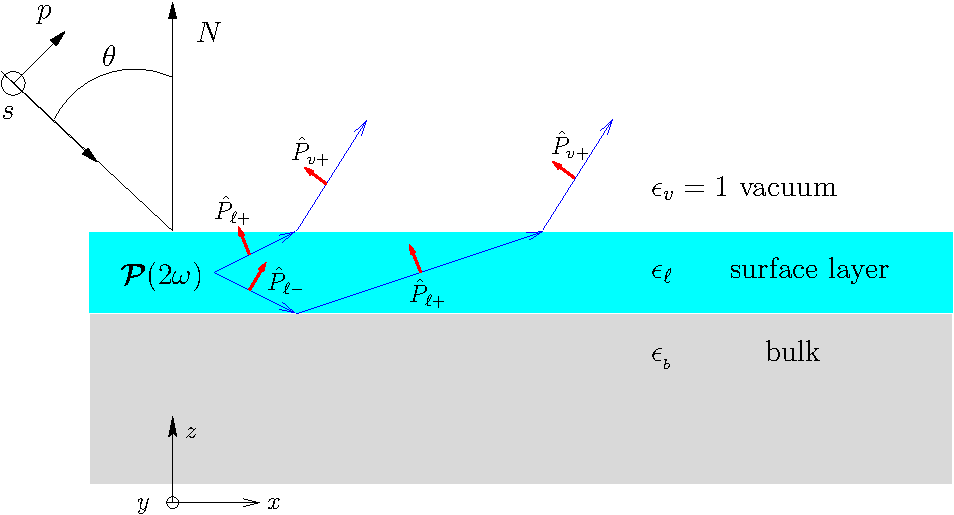
\includegraphics[scale=.5]{figures/diag-3layer}
\caption{Representation of the 3-layer model for SSHG. The vacuum region is on
top with $\varepsilon_{v}=1$; the layer with nonlinear polarization
$\mathcal{P}^{\mathrm{a}}(2\omega) = \chi^{\mathrm{abc}}(-2\omega;\omega,\omega)
E^{\mathrm{b}}(\omega)E^{\mathrm{c}}(\omega)$ is characterized with
$\varepsilon_{\ell}(\omega)$, and the bulk with $\varepsilon_{b}(\omega)$. In
the dipole approximation, the bulk does not radiate SH for centrosymmetric
materials.}
\label{fig:3layer}
\end{figure}

To model the electromagnetic response of the 3-layer model, we follow Ref.
\cite{mizrahiJOSA88} and assume a polarization sheet of the form
\begin{align}\label{m31}
\mathbf{P}(\mathbf{r},t) = \boldsymbol{\mathcal{P}}
  e^{i\boldsymbol{\kappa}\cdot\mathbf{R}}e^{-i\omega t}\delta(z - z_{\beta}) 
+ \mathrm{c.c.},
\end{align}
where $\mathbf{R}=(x,y)$, $\boldsymbol{\kappa}$ is the component of the wave
vector $\boldsymbol{\nu}_{\beta}$ parallel to the surface, and
$z_{\beta}$ is the position of the sheet within medium $\beta$. In Ref.
\cite{sipeJOSAB87} they demonstrate that the solution of the Maxwell equations
for the radiated fields $E_{\beta,p\pm}$, and $E_{\beta,s}$ with
$\mathbf{P}(\mathbf{r},t)$ as a source can be written, at points $z\neq 0$, as
\begin{equation}\label{r2}
(E_{\beta,p\pm},E_{\beta,s}) = 
(\frac{\gamma i\tilde\omega^2}{\tilde w_{\beta}}
\,\hat{\mathbf{p}}_{\beta\pm}\cdot\boldsymbol{\mathcal{P}},
\frac{\gamma i\tilde\omega^2}{\tilde w_{\beta}}
\,\hat{\mathbf{s}}\cdot\boldsymbol{\mathcal{P}}),
\end{equation} 
where $\gamma=2\pi$ in CGS units or $\gamma=1/2\epsilon_{0}$ in MKS units, and
$\tilde\omega=\omega/c$. Also, $\hat{\mathbf{s}}$ and
$\hat{\mathbf{p}}_{\beta\pm}$ are the unitary vectors for the $s$ and $p$
polarizations of the radiated field, respectively. The $\pm$ refers to upward
($+$) or downward ($-$) direction of propagation within medium $\beta$, as shown
in Fig. \ref{fig:MR3layer}. Also, $\tilde{w}_{\beta}(\omega)=\tilde{\omega}
w_{\beta}$, where
\begin{equation}\label{r3}
w_{\beta}(\omega) = 
\big(\epsilon_{\beta}(\omega) - \sin^{2}\theta_{0}\big)^{1/2},
\end{equation}
where $\theta_{0}$ is the angle of incidence of $\mathbf{E}_{v}(\omega)$, 
and
\begin{equation}\label{r4}
\hat{\mathbf{p}}_{\beta\pm}(\omega) =
\frac{\kappa(\omega)\hat{\mathbf{z}}\mp 
     \tilde{w}_{\beta}(\omega)\hat{\boldsymbol{\kappa}}} 
{\tilde\omega n_{\beta}(\omega)}
=
\frac{\sin\theta_{0}\hat{\mathbf{z}}\mp 
  w_{\beta}(\omega)\hat{\boldsymbol{\kappa}}} 
{n_{\beta}(\omega)}
,
\end{equation}
where $\kappa(\omega)=|\boldsymbol{\kappa}|=\tilde\omega\sin\theta_{0}$, $n_{\beta}(\omega)=\sqrt{\epsilon_{\beta}(\omega)}$ is the index of refraction of medium $\beta$, and $z$ is the direction perpendicular to the surface that points towards the vacuum. We chose the plane of incidence along the $\boldsymbol{\kappa}z$ plane, then
\begin{equation}\label{mc1}
\hat{\boldsymbol{\kappa}}
= \cos\phi\hat{\mathbf{x}} + \sin\phi\hat{\mathbf{y}},
\end{equation}
and
\begin{equation}\label{mmc2}
\hat{\mathbf{s}} = -\sin\phi\hat{\mathbf{x}} + \cos\phi\hat{\mathbf{y}},
\end{equation}
where $\phi$ the angle with respect to the $x$ axis.

In the three-layer model the nonlinear polarization responsible for the second harmonic generation (SHG) is immersed in the thin $\beta=\ell$ layer, and is given by
\begin{equation}\label{tres}
\mathcal{P}_i(2\omega)=
\left\{
\begin{array}{cc}
\chi_{ijk}(2\omega)E_{j}(\omega)E_{k}(\omega) & \text{(CGS units)} \\
\epsilon_{0}\chi_{ijk}(2\omega)E_{j}(\omega)E_{k}(\omega) & \text{(MKS units)}
\end{array}
\right.
,
\end{equation}
where the tensor $\boldsymbol{\chi}(2\omega)$ is the surface nonlinear dipolar susceptibility and the Cartesian indices $i,j,k$ are summed if repeated. Also, $\chi_{ijk}(2\omega)=\chi_{ikj}(2\omega)$ is the intrinsic permutation symmetry due to the fact that SHG is degenerate in $E_j(\omega)$ and $E_k(\omega)$. As it was done in Ref. \cite{mizrahiJOSA88}, in presenting the results Eq.~\eqref{r2}-\eqref{mmc2} we have taken the polarization sheet (Eq.~\eqref{m31}) to be oscillating at some frequency $\omega$. However, in the following we find it convenient to use $\omega$ exclusively to denote the fundamental frequency and $\boldsymbol{\kappa}$ to denote the component of the incident wave vector parallel to the surface. Then the nonlinear generated polarization is oscillating at $\Omega= 2\omega$ and will be characterized by a wave vector parallel to the surface $\mathbf{K}=2\boldsymbol{\kappa}$. We can carry over Eqs. \eqref{m31}-\eqref{mmc2} simply by replacing the lowercase symbols ($\omega,\tilde\omega,\boldsymbol{\kappa},n_{\beta},\tilde w_{\beta},w_{\beta},\hat{\mathbf{p}}_{\beta\pm},\hat{\mathbf{s}}$) with uppercase symbols ($\Omega,\tilde\Omega,\mathbf{K},N_{\beta},\tilde W_{\beta},W_{\beta},\hat{\mathbf{P}}_{\beta\pm},\hat{\mathbf{S}}$), all evaluated at $2\omega$ and we always have $\hat{\mathbf{S}}=\hat{\mathbf{s}}$.

\begin{figure}[t]
\centering 
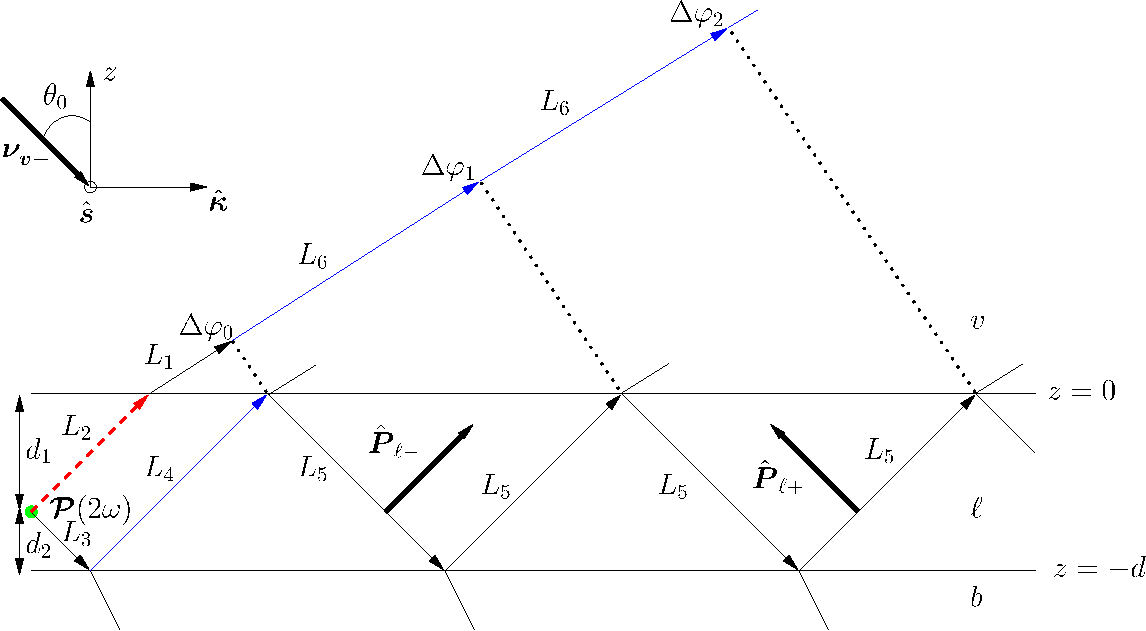
\includegraphics[scale=.5]{figures/diag-3layer_MR_2w}
\caption{Sketch of the three layer model for SHG. Vacuum ($v$) is on top with $\epsilon_v=1$; the layer $\ell$, of thickness $d=d_1+d_2$, is characterized with $\epsilon_{\ell}(\omega)$, and it is where the SH polarization sheet $\boldsymbol{\mathcal{P}}(2\omega)$ is located at $z_\ell=d_1$; The bulk $b$ is described with $\epsilon_{b}(\omega)$. The arrows point along the direction of propagation, and the $p$-polarization unit vector, $\hat{\mathbf{P}}_{\ell -(+)}$, along the downward (upward) direction is denoted with a thick arrow. The $s$-polarization unit vector $\hat{\mathbf{s}}$, points out of the page. The fundamental field $\mathbf{E}(\omega)$ is incident from the vacuum side along the $z\hat{\boldsymbol{\kappa}}$-plane, with $\theta_{0}$ its angle of incidence and $\boldsymbol{\nu}_{v-}$ its wave vector. $\Delta\varphi_{i}$ denote the phase difference of the multiply reflected beams with respect to the first vacuum transmitted beam (dashed-red arrow), where the dotted lines are perpendicular to this beam (see the text for details).}
\label{fig:MR3layer}
\end{figure}

To describe the propagation of the SH field, we  see from
Fig. \ref{fig:MR3layer}, that it is refracted at the 
layer-vacuum interface ($\ell v$), and multiply reflected from the
layer-bulk ($\ell b$)
and layer-vacuum ($\ell v$)
interfaces, thus we can define,
\begin{equation}\label{r5}
\mathbf{T}^{\ell v}
= \hat{\mathbf{s}}T_s^{\ell v}\hat{\mathbf{s}} 
+ \hat{\mathbf{P}}_{v+}T_{p}^{\ell v} \hat{\mathbf{P}}_{\ell +},
\end{equation}
as the tensor for transmission from $\ell v$ interface,
\begin{equation}\label{r6}
\mathbf{R}^{\ell b}
= \hat{\mathbf{s}}R_s^{\ell b}\hat{\mathbf{s}}
+ \hat{\mathbf{P}}_{\ell +}R_{p}^{\ell b} \hat{\mathbf{P}}_{\ell -},
\end{equation} 
as the tensor of reflection from the $\ell b$ interface, 
and
\begin{equation}\label{r6b}
\mathbf{R}^{\ell v}
= \hat{\mathbf{s}}R_s^{\ell v}\hat{\mathbf{s}}
+ \hat{\mathbf{P}}_{\ell -}R_{p}^{\ell v} \hat{\mathbf{P}}_{\ell +},
\end{equation} 
as that of the $\ell v$ interface. 
The Fresnel factors in uppercase letters, $T^{ij}_{s,p}$ and $R^{ij}_{s,p}$,
are evaluated at $2\omega$  from the following well known formulas 
\begin{equation}\label{e.f1}
\begin{split}
t_s^{ij}(\omega) &=
\frac{2k_{i}(\omega)}{k_{i}(\omega)+k_{j}(\omega)},
\quad\quad  
t_{p}^{ij}(\omega) =
\frac{2k_{i}(\omega)\sqrt{\epsilon_{i}(\omega)\epsilon_j(\omega)}}
     {k_{i}(\omega)\epsilon_{j}(\omega)+k_{j}(\omega)\epsilon_{i}(\omega)},\\
r_s^{ij}(\omega) &=
\frac{k_{i}(\omega) - k_{j}(\omega)}
     {k_{i}(\omega) + k_{j}(\omega)},
\quad\quad 
r_{p}^{ij}(\omega) =
\frac{k_{i}(\omega)\epsilon_{j}(\omega) - k_{j}\epsilon_{i}(\omega)}
     {k_{i}(\omega)\epsilon_{j}(\omega) + k_{j}(\omega)\epsilon_{i}(\omega)}. 
\end{split}
\end{equation}
From these expressions one can show that,
\begin{align}\label{mf}
1 + r^{\ell b}_{s} &= t^{\ell b}_{s}\nonumber\\
1 + r^{\ell b}_{p}
&= \frac{n_b}{n_\ell}
t^{\ell b}_{p} 
\nonumber\\
1 - r^{\ell b}_{p}
&= \frac{n_\ell}{n_b}
   \frac{w_{b}}{w_{\ell}}t^{\ell b}_{p}\\
t^{\ell v}_{p} &= \frac{w_{\ell}}{w_{v}}t^{v\ell}_{p}\nonumber\\
t^{\ell v}_{s} &= \frac{w_{\ell}}{w_{v}}t^{v\ell}_{s}\nonumber 
.
\end{align}


\subsection{Multiple SH reflections}

The SH field $\mathbf{E}(2\omega)$ radiated by the SH polarization 
$\boldsymbol{\mathcal{P}}(2\omega)$
will radiate directly into vacuum and also into the bulk,
where it will be reflected back at the thin-layer-bulk interface into 
the thin layer again and this beam will be multiple-transmitted and 
reflected as shown in Fig.~\ref{fig:MR3layer}. 
As the two beams propagate a phase difference will develop between
them, according to
\begin{align}\label{m99}
\Delta\varphi_m&=\tilde\Omega\Big((L_{3} + L_{4} + 2mL_{5})N_{\ell}
-\big(L_{2}N_{\ell} + (L_{1} + mL_{6})N_{v}\big)
\Big)
\nonumber\\
&=\delta_{0} + m\delta\quad m=0,1,2,\ldots
,
\end{align}
where
\begin{align}\label{m97}
\delta_{0}=8\pi\left(\frac{d_2}{\lambda_0}\right)\sqrt{n^2_\ell(2\omega)-\sin^2\theta_{0}}
,
\end{align}
\begin{align}\label{m96}
\delta=8\pi\left(\frac{d}{\lambda_0}\right)\sqrt{n^2_\ell(2\omega)-\sin^2\theta_{0}}
,
\end{align}
where $\lambda_0$ is the wavelength of the fundamental field in
vacuum, $d$ the thickness of layer $\ell$ and $d_2$ the distance of
$\boldsymbol{\mathcal{P}}(2\omega)$  
from the $\ell b$ interface 
(see Fig.~\ref{fig:MR3layer}).
We see that
$\delta_{0}$ is the phase difference of 
the first and second transmitted beams, and $m\delta$ that of the first 
and  third ($m=1$), fourth ($m=2$), etc. beams (see 
Fig.~\ref{fig:MR3layer}). 

To take into account the multiple reflections of the generated SH
field in the layer $\ell$, we proceed as follows. We show the algebra
for the $p$-polarized SH field, the $s$-polarized field could be
worked out along the same steps. The multiple-reflected $\mathbf{E}_p(2\omega)$
field is given by
\begin{equation}\label{m7}
\begin{split}
\mathbf{E}(2\omega) 
&=  
  E_{p+}(2\omega)\mathbf{T}^{\ell v}\cdot\hat{\mathbf{P}}_{\ell +}
+ E_{p-}(2\omega)\mathbf{T}^{\ell v}
\cdot\mathbf{R}^{\ell b}\cdot\hat{\mathbf{P}}_{\ell-}e^{i\Delta\varphi_{0}}
+ E_{p-}(2\omega)\mathbf{T}^{\ell v}
\cdot\mathbf{R}^{\ell b}\cdot\mathbf{R}^{\ell v}
\cdot\mathbf{R}^{\ell b}\cdot\hat{\mathbf{P}}_{\ell-}e^{i\Delta\varphi_{1}}
\\
&
+ E_{p-}(2\omega)\mathbf{T}^{\ell v}
\cdot\mathbf{R}^{\ell b}\cdot\mathbf{R}^{\ell v}
\cdot\mathbf{R}^{\ell b}\cdot\mathbf{R}^{\ell v}
\cdot\mathbf{R}^{\ell b}\cdot\hat{\mathbf{P}}_{\ell-}e^{i\Delta\varphi_{2}}
+\cdots 
\\
&= 
E_{p+}(2\omega)\mathbf{T}^{\ell v}\cdot\hat{\mathbf{P}}_{\ell +}
+ E_{p-}(2\omega) \mathbf{T}^{\ell v}
\cdot\sum_{m=0}^\infty  
\big(
\mathbf{R}^{\ell b}\cdot\mathbf{R}^{\ell v} 
e^{i\delta}\Big)^m 
\cdot\mathbf{R}^{\ell b}\cdot\hat{\mathbf{P}}_{\ell-}e^{i\delta_{0}}
.
\end{split}
\end{equation} 
From Eqs.~\eqref{r5}-\eqref{r6b} is easy to show
that
\begin{align}\label{m1}
\mathbf{T}^{\ell v}\cdot 
\Big(\mathbf{R}^{\ell b}\cdot\mathbf{R}^{\ell v}\Big)^n 
\cdot \mathbf{R}^{\ell b}
&=
\hat{\mathbf{s}}
T^{\ell v}_s\Big(R^{\ell b}_sR^{\ell v}_s\Big)^n 
 R^{\ell b}_s 
\hat{\mathbf{s}}
+
\hat{\mathbf{P}}_{v+}
T^{\ell v}_p\Big(R^{\ell b}_pR^{\ell v}_p\Big)^n 
 R^{\ell b}_p 
\hat{\mathbf{P}}_{\ell-}
,
\end{align}
then,
\begin{equation}\label{m7}
\begin{split}
\mathbf{E}(2\omega) 
&= 
\hat{\mathbf{P}}_{\ell +}T^{\ell v}_p
\Big(
E_{p+}(2\omega) 
+
\frac{R^{\ell b}_pe^{i\delta_{0}}}{1+R^{v\ell}_pR^{\ell b}_pe^{i\delta}}
E_{p-}(2\omega) 
\Big)
,
\end{split}
\end{equation}
where we used $R^{ij}_{s,p}=-R^{ji}_{s,p}$.
Using Eq.~\eqref{r2}, we can readily write
\begin{equation}\label{mr8}
\mathbf{E}(2\omega) = \frac{\gamma i\tilde{\Omega}}{W_{\ell}}
\mathbf{H}_{\ell}\cdot\boldsymbol{\mathcal{P}}(2\omega),
\end{equation}
where
\begin{equation}\label{mr9}
\mathbf{H}_{\ell}
= \hat{\mathbf{s}}\,T_s^{\ell v}
\left(1+
R^M_s
\right)
\hat{\mathbf{s}}
+ \hat{\mathbf{P}}_{v+}T_{p}^{\ell v}
\left(
\hat{\mathbf{P}}_{\ell +} +
R^M_p
 \hat{\mathbf{P}}_{\ell -}
\right). 
\end{equation}
and
\begin{align}\label{m61}
R^M_l\equiv\frac{R^{\ell b}_le^{i\delta_{0}}}{1+R^{v\ell}_l R^{\ell b}_l e^{i\delta}}
\quad l=s,p
,
\end{align}
is defined as the multiple ($M$) reflection coefficient.
To make touch with the work of Ref. \cite{mizrahiJOSA88} where
$\boldsymbol{\mathcal{P}}(2\omega)$ is located on top of the
vacuum-surface interface and only the vacuum radiated beam and the
first (and only) reflected beam need to be considered, we take
$\ell=v$ and $d_2=0$, then 
$T^{\ell v}=1$, $R^{v\ell}=0$ and $\delta_{0}=0$, with which
$R^M_l=R^{vb}_l$. 
Thus, Eq.~\eqref{mr9} coincides with Eq. (3.8) of
Ref. \cite{mizrahiJOSA88}. 

\subsection{Multiple reflections for the linear field}
\begin{figure}[t]
\centering 
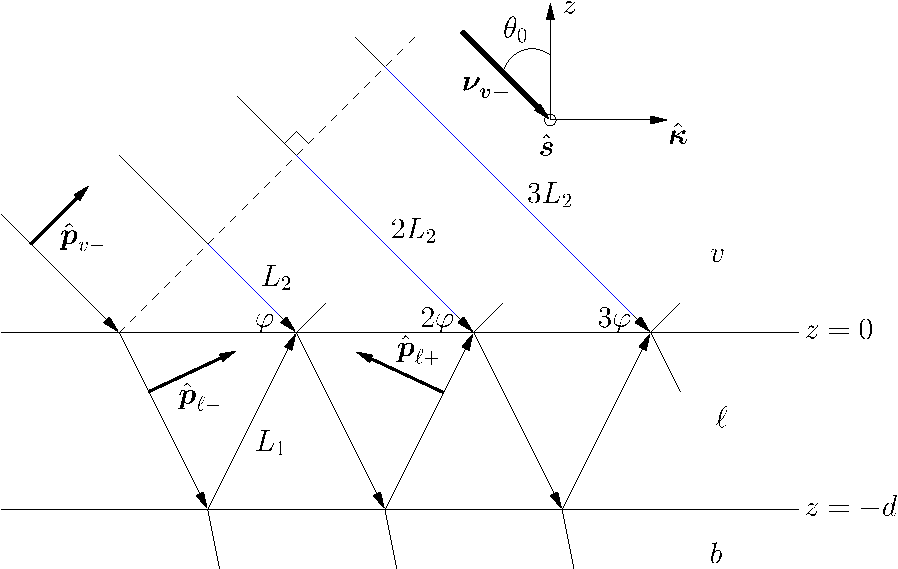
\includegraphics[scale=.5]{figures/diag-3layer_MR_1w}
\caption{(color on line) Sketch for the multiple reflected  fundamental field
$\mathbf{E}(\omega)$, which impinges from the vacuum side along the
$z\hat{\boldsymbol{\kappa}}$-plane, with $\theta_{0}$ and $\boldsymbol{\nu}_{v-}$
its angle of incidence and wave vector, respectively. The arrows point along the
direction of propagation. The $p$-polarization unit vectors, $\hat{\mathbf{p}}_{\beta
\pm}$, along the downward (-) or upward (+) direction are denoted with thick
arrows, where $\beta=v$ or $\ell$. The $s$-polarization unit vector $\hat{\mathbf{s}}$
points out of the page, and $(1,2,3,\dots)\phi$ denotes the phase difference for
the multiply reflected beams with respect to the incident field, where the
dotted line is perpendicular to this beam (see the text for
details).\label{linear}}
\end{figure}

Similar to the SH field, here we consider the multiple reflections of
the fundamental field $\mathbf{E}(\omega)$ inside the thin $\ell$ layer.
In Fig.~\ref{linear} we show the situation where $\mathbf{E}(\omega)$
impinges from the vacuum side with an angle of incidence $\theta_{0}$. 
As the first transmitted beam is multiply reflected from the $\ell b$ and the
$\ell v$ interfaces, it accumulates a phase difference of $n\phi$,
with $n=1,2,3,\ldots$, given by
\begin{align}\label{mphi}
\phi&=\frac{\omega}{c}(2L_1n_\ell-L_2n_v)
\nonumber\\
&=4\pi\left(\frac{d}{\lambda_0}\right)\sqrt{n^2_\ell-\sin^2\theta_{0}}
,
\end{align}
where $n_v=1$. Besides the equivalent of Eqs.~\eqref{r6} and
\eqref{r6b}, for $\omega$, we also need
\begin{align}\label{mvv}
\mathbf{t}^{v\ell}
= \hat{\mathbf{s}}t_s^{v\ell}\hat{\mathbf{s}} 
+ \hat{\mathbf{p}}_{\ell -}t_{p}^{v\ell} \hat{\mathbf{p}}_{v -}
,
\end{align}
to write
\begin{align}\label{mcvew}
\mathbf{E}(\omega)
&=E_{0}\Big[
\mathbf{t}^{v\ell}
+
\mathbf{r}^{\ell b}\cdot\mathbf{t}^{v\ell}e^{i\phi}
+
\mathbf{r}^{\ell b}\cdot\mathbf{r}^{\ell v}\cdot \mathbf{r}^{\ell b}\cdot\mathbf{t}^{v\ell} e^{i2\phi}
+
\mathbf{r}^{\ell b}\cdot\mathbf{r}^{\ell v}\cdot 
\mathbf{r}^{\ell b}\cdot\mathbf{r}^{\ell v}
\cdot \mathbf{r}^{\ell b}\cdot\mathbf{t}^{v\ell} e^{i3\phi}
+\cdots\Big]\cdot\mathbf{e}^{\mathrm{in}}
\nonumber\\
&=E_{0}\Big[
1
+
\Big(1+
\mathbf{r}^{\ell b}\cdot\mathbf{r}^{\ell v}e^{i\phi}
+
(\mathbf{r}^{\ell b}\cdot\mathbf{r}^{\ell v})^2e^{i2\phi}+\cdots
\Big)\cdot
\mathbf{r}^{\ell b}e^{i\phi}
\Big]\cdot \mathbf{t}^{v\ell}\cdot\mathbf{e}^{\mathrm{in}}
\nonumber\\
&=
E_{0}\Big[\hat{\mathbf{s}} t^{v\ell}_s(1+r^M_s)\hat{\mathbf{s}}
+
t^{v\ell}_p\left(\hat{\mathbf{p}}_{\ell-}+\hat{\mathbf{p}}_{\ell+}r^{M}_p
\right)\hat{\mathbf{p}}_{v-}
\Big]\cdot\mathbf{e}^{\mathrm{in}}
\end{align}
where
\begin{align}\label{mvrm}
r^M_l=\frac{r^{\ell b}_le^{i\phi}}{1+r^{v\ell}_lr^{\ell
  b}_le^{i\phi}}\quad l=s,p
.
\end{align}
We define $\mathbf{E}^{l}(\omega)\equiv E_{0}\mathbf{e}^{\omega,l}_\ell$ ($l=s,p$),
where using Eq.~\eqref{r4}, we obtain that
\begin{eqnarray}\label{mcvep}
\mathbf{e}^{\omega,p}_{\ell}=\frac{t^{v\ell}_p}{n_\ell}
\left( 
r^{M+}_p\sin\theta_{0}\hat{\mathbf{z}}
+ 
r^{M-}_pw_\ell\hat{\boldsymbol{\kappa}}
\right)  
,
\end{eqnarray} 
for $p$-input polarization, i.e. $\mathbf{e}^{\mathrm{in}}=\hat{\mathbf{p}}_{v-}$, 
and
\begin{eqnarray}\label{mcvep}
\mathbf{e}^{\omega,s}_\ell=t^{v\ell}_sr^{M+}_s\hat{\mathbf{s}}
,
\end{eqnarray}
for $s$-input polarization, i.e. $\mathbf{e}^{\mathrm{in}}=\hat{\mathbf{s}}$,
where
\begin{eqnarray}\label{mvc}
r^{M\pm}_l=1\pm r^M \quad l=s,p.
\end{eqnarray}
\subsection{SHG Yield}

The magnitude of the radiated field is given by
$E(2\omega)=\hat{\mathbf{e}}^{\mathrm{out}}\cdot\mathbf{E}(2\omega)$, where
$\hat{\mathbf{e}}^{\mathrm{out}}$ is the polarization vector of the radiated
field, for instance $\hat{\mathbf{s}}$ or $\hat{\mathbf{P}}_{v+}$. Then, we
write
\begin{equation}\label{m1}
\begin{split}
\hat{\mathbf{P}}_{\ell +} + R^M_p\hat{\mathbf{P}}_{\ell -}
&= \frac{\sin\theta_{0}\hat{\mathbf{z}} - W_{\ell}\hat{\boldsymbol{\kappa}}}
        {N_{\ell}}
 + R^M_p
   \frac{\sin\theta_{0}\hat{\mathbf{z}} + W_{\ell}\hat{\boldsymbol{\kappa}}}
        {N_{\ell}}
\\
&= \frac{1}{N_{\ell}}
\left(
\sin\theta_{0}R^M_{p+}\hat{\mathbf{z}}
- K_{\ell}R^M_{p-}\hat{\boldsymbol{\kappa}}
\right)
,
\end{split}
\end{equation}
where
\begin{align}\label{rm}
R^{M\pm}_l\equiv 1 \pm R^M_l \quad l=s,p
.
\end{align}
 Using Eq.~\eqref{mf}
 we write Eq.~\eqref{mr8} as
\begin{equation}\label{r10}
E(2\omega) = \frac{2\gamma i \omega}{cW_\ell}
\hat{\mathbf{e}}^{\mathrm{out}}\cdot 
\mathbf{H}_{\ell}\cdot 
\boldsymbol{\mathcal{P}}(2\omega) 
= \frac{2\gamma i \omega}{cW_v}
 \mathbf{e}^{\,2\omega}_{\ell}\cdot\boldsymbol{\mathcal{P}}(2\omega). 
\end{equation}
\begin{equation}\label{r12mm}
\begin{split}
\mathbf{e}^{2\omega}_{\ell} &=\hat{\mathbf{e}}^{\mathrm{out}}\cdot 
\Bigg[
\hat{\mathbf{s}}T_{s}^{v\ell}R^{M+}_s\hat{\mathbf{s}} + 
\hat{\mathbf{P}}_{v+}
\frac{T^{v\ell}_{p}}
     {N_\ell}
\left(
\sin\theta_{0}R^{M+}_p\hat{\mathbf{z}}
- W_{\ell}R^{M-}_p\hat{\boldsymbol{\kappa}}
\right) 
\Bigg]
. 
\end{split}
\end{equation}  
 We pause here to reduce above result to the case where the nonlinear
polarization $\mathbf{P}(2\omega)$ radiates from vacuum instead from the layer
$\ell$. For such case we simply take $\epsilon_{\ell}(2\omega)=1$ and $\ell=v$
($T^{\ell v}_{s,p}=1$), to get
\begin{equation}\label{r13}
\mathbf{e}^{\,2\omega}_{v} = \hat{\mathbf{e}}^{\mathrm{out}}
\cdot\left[
\hat{\mathbf{s}}T_s^{v b}\hat{\mathbf{s}} + \hat{\mathbf{P}}_{v+}
\frac{T^{v b}_{p}}{\sqrt{\epsilon_{b}(2\omega)}}
\left(
  \epsilon_{b}(2\omega)\sin\theta_{0}\hat{\mathbf{z}}
  - W_{b}\hat{\boldsymbol{\kappa}}
\right) 
\right] 
,
\end{equation}
which agrees with Eq. (3.10) of Ref. \cite{mizrahiJOSA88}.

In the three layer model the SH polarization $\boldsymbol{\mathcal{P}}(2\omega)$ is located in layer $\ell$,
where we evaluate the fundamental field required in Eq. \eqref{tres}.
We write
\begin{equation}\label{m2}
\mathbf{E}_{\ell}(\omega)=E_{0}\left(
\hat{\mathbf{s}} t^{v\ell}_s(1+r^{\ell b}_s)\hat{\mathbf{s}}
+
\hat{\mathbf{p}}_{\ell-}
 t^{v\ell}_{p}
\hat{\mathbf{p}}_{v-}
+
\hat{\mathbf{p}}_{\ell+}
t^{v\ell}_{p}r^{\ell b}_{p}
\hat{\mathbf{p}}_{v-}
\right)\cdot\hat{\mathbf{e}}^{\mathrm{in}}=E_{0}\mathbf{e}^\omega_{\ell}
,
\end{equation} 
where $\mathbf{e}^{\mathrm{in}}$ is the $s$ ($\hat{\mathbf{s}}$) or $p$
($\hat{\mathbf{p}}_{v-}$)
incoming polarization of
the fundamental electric field. 
Above field is composed of the transmitted field and its first
reflection from the $\ell b$ interface for $s$ and $p$ polarizations.
The fundamental field, once inside the layer $\ell$ will be multiply
reflected at the $\ell v$ and $\ell b$ interfaces, however each
reflection will diminish the intensity of the fundamental field, and as the SHG
yield goes with the square of this field, the contribution of the
subsequent reflections, other than the one considered in
Eq.~\eqref{m2},  could be safely neglected.
From Eq.~\eqref{mf}
we find that
\begin{equation}\label{m12}
\mathbf{e}^{\omega}_{\ell}
= \left[
\hat{\mathbf{s}}t_{s}^{v\ell}t_{s}^{\ell b}\hat{\mathbf{s}} 
+ \frac{t^{v\ell}_{p}t^{\ell b}_{p}}
       {n^2_\ell n_b}
\left(
  n^2_b
\sin\theta_{0}\hat{\mathbf{z}}
+ n^2_\ell w_b\hat{\boldsymbol{\kappa}}
\right)
\hat{\mathbf{p}}_{v-}
\right]
\cdot\hat{\mathbf{e}}^{\mathrm{in}}.  
\end{equation}  
Again, to touch base with Ref. \cite{mizrahiJOSA88},
if we would like to evaluate the fields in the bulk, instead of the layer
$\ell$, we simply take 
$n_\ell=n_b,\,(t^{\ell b}_{s,p}=1$), to obtain
\begin{equation}\label{m13}
\mathbf{e}^{\omega}_{b}
= \left[
\hat{\mathbf{s}}t_{s}^{vb}\hat{\mathbf{s}}
+ \frac{t^{vb}_{p}}{n_b}
\left(
\sin\theta_{0}\hat{\mathbf{z}} + w_b\hat{\boldsymbol{\kappa}}
\right) 
\hat{\mathbf{p}}_{v-}
\right]
\cdot\hat{\mathbf{e}}^{\mathrm{in}},  
\end{equation} 
that is in agreement with Eq. (3.5) of Ref. \cite{mizrahiJOSA88}.
Then,
 we can write Eq. \eqref{tres} as
\begin{equation}\label{m4}
\boldsymbol{\mathcal{P}}(2\omega) = 
\left\{
\begin{array}{cc}  
E^{2}_{0}\,\boldsymbol{\chi}:\mathbf{e}^{\omega}_{\ell}\mathbf{e}^{\omega}_{\ell}
& \text{(CGS units)} \\
\epsilon_{0}E^{2}_{0}\,\boldsymbol{\chi}:\mathbf{e}^{\omega}_{\ell}\mathbf{e}^{\omega}_{\ell}
& \text{(MKS units)} \\
\end{array}
\right.
,
\end{equation}
where $E_{0}$ is the intensity of the fundamental electric field.
Finally, with above equation we write Eq.~\eqref{r10} as
\begin{equation}\label{mr10}
E(2\omega) 
= \frac{2\eta i \omega}{cW_v}
\mathbf{e}^{2\omega}_{\ell}\cdot\boldsymbol{\chi}:\mathbf{e}^{\omega}_{\ell}
\mathbf{e}^{\omega}_{\ell}
,
\end{equation}
where $\eta=2\pi$ for CGS units and $\eta=1/2$ for MKS units.
To ease on the notation, we define
\begin{align}\label{mc0}
\Upsilon_{\mathrm{iO}}
\equiv 
\mathbf{e}^{2\omega}_{\ell}\cdot\boldsymbol{\chi}:\mathbf{e}^{\omega}_{\ell}
\mathbf{e}^{\omega}_{\ell}
,
\end{align}
where i stands for the incoming polarization of the fundamental
electric field given by $\hat{\mathbf{e}}^{\mathrm{in}}$ in Eq.~\eqref{m12},
and O for the outgoing polarization of the SH electric field
given by $\hat{\mathbf{e}}^{\mathrm{out}}$ in Eq.~\eqref{r12mm}.

From Eqs. \eqref{uno} and \eqref{dos} we obtain that
in the CGS units ($\eta=2\pi$)
\begin{align}\label{r01}
|E(2\omega)|^2 
&= |E_{0}|^4\frac{16\pi^{2}\omega^{2}}{c^{2}W^2_v}
\left\vert  
\Upsilon_{\mathrm{iO}}
\right\vert^{2}
\nonumber\\
\frac{c}{2\pi}|\sqrt{N_v}E(2\omega)|^{2} 
&=
\frac{32\pi^{3}\omega^{2}}{c^{3}\cos^2\theta_{0}}
\left\vert  
\frac{\sqrt{N_v}}{n^2_\ell}
\Upsilon_{\mathrm{iO}}
\right\vert^{2} 
\left(\frac{c}{2\pi}|\sqrt{n_\ell}E_{0}|^{2}\right)^{2},
\nonumber\\ 
I(2\omega) 
&= \frac{32\pi^{3}\omega^{2}}{c^{3}\cos^2\theta_{0}}
\left\vert  
\frac{\sqrt{N_v}}{n^2_\ell}
\Upsilon_{\mathrm{iO}}
\right\vert^{2}I^{2}(\omega),
\nonumber\\
\mathcal{R}_{\mathrm{iO}}(2\omega) 
&= 
\frac{32\pi^{3}\omega^{2}}{c^{3}\cos^2\theta_{0}}
\left\vert  
\frac{1}{n_\ell}
\Upsilon_{\mathrm{iO}}
\right\vert^{2}
,
\end{align} 
and in MKS units ($\eta=1/2$)
\begin{align}\label{r01m}
|E(2\omega)|^2 
&= |E_{0}|^4
\frac{\omega^{2}}{c^{2}W^2_v}
\left\vert  
\Upsilon_{\mathrm{iO}}
\right\vert^{2}
\nonumber\\
2\epsilon_{0}c|\sqrt{N_v}E(2\omega)|^{2} 
&=
\frac{2\epsilon_{0}\omega^{2}}{c\cos^2\theta_{0}}
\left\vert  
\frac{\sqrt{N_v}}{n^2_\ell}
\Upsilon_{\mathrm{iO}}
\right\vert^{2} 
\frac{1}{4\epsilon^2_0c^2}\left(2\epsilon_{0}c|\sqrt{n_\ell}E_{0}|^{2}\right)^{2},
\nonumber\\ 
I(2\omega) 
&= 
\frac{\omega^{2}}{2\epsilon_{0}c^3\cos^2\theta_{0}}
\left\vert  
\frac{\sqrt{N_v}}{n^2_\ell}
\Upsilon_{\mathrm{iO}}
\right\vert^{2}I^{2}(\omega),
\nonumber\\
\mathcal{R}_{\mathrm{iO}}(2\omega) 
&= \frac{\omega^{2}}{2\epsilon_{0}c^3\cos^2\theta_{0}}
\left\vert  
\frac{1}{n_\ell}
\Upsilon_{\mathrm{iO}}
\right\vert^{2} 
,
\end{align} 
\begin{equation}\label{mc6}
\mathcal{R}_{\mathrm{iO}}(2\omega) 
\left\{
\begin{array}{cc} 
\frac{32\pi^{3}\omega^{2}}{c^{3}\cos^2\theta_{0}}
\left\vert  
\frac{1}{n_\ell}
\Upsilon_{\mathrm{iO}}
\right\vert^{2} 
& \text{(CGS units)} \\
\frac{\omega^{2}}{2\epsilon_{0}c^3\cos^2\theta_{0}}
\left\vert  
\frac{1}{n_\ell}
\Upsilon_{\mathrm{iO}}
\right\vert^{2} 
& \text{(MKS units)} 
\end{array}
\right.
,
\end{equation}
as the SHG yield, where $N_v=1$ and $W_v=\cos\theta_{0}$.
In the MKS unit system $\boldsymbol{\chi}$ is given in m$^2$/V, since
it is a surface second order nonlinear susceptibility, and
$\mathcal{R}_{\mathrm{iO}}$ is given in m$^2$/W. 


\verb=tal vez esto al apendice=
At this point we mention that to recover the results of Ref.
\cite{mizrahiJOSA88} which are equivalent of those of Ref. \cite{sipePRB87}, we
take $\mathbf{e}^{2\omega}_{\ell}\to \mathbf{e}^{2\omega}_v$,
$\mathbf{e}^{\omega}_{\ell}\to \mathbf{e}^{\omega}_{b}$, 
and then
\begin{equation}\label{m69}
\mathcal{R}(2\omega) =
\frac{32\pi^{3} \omega^{2}}{c^{3}\cos^{2}\theta_{0}}
\left\vert
\mathbf{e}^{\,2\omega}_{v}\cdot\boldsymbol{\chi}:
\mathbf{e}^{\omega}_{b}\mathbf{e}^{\omega}_{b}
\right\vert^{2} 
,
\end{equation}
will give the SHG yield of a nonlinear polarization sheet radiating from vacuum
on top of the surface and where the fundamental field is evaluated below the
surface that is characterized by $\epsilon_{b}(\omega)$.


\section{One SH Reflection}
Therefore, the total radiated field at 
$2\omega$ is 
\begin{equation}\label{r7}
\begin{split}
\mathbf{E}(2\omega)  
&= E_s(2\omega)  
\left(
\mathbf{T}^{\ell v} + \mathbf{T}^{\ell v}\cdot\mathbf{R}^{\ell b}
\right)  
\cdot\hat{\mathbf{s}}\nonumber\\
&+ E_{p+}(2\omega)\mathbf{T}^{\ell v}\cdot\hat{\mathbf{P}}_{\ell +}
 + E_{p-}(2\omega)\mathbf{T}^{\ell v}
\cdot\mathbf{R}^{\ell b}\cdot\hat{\mathbf{P}}_{\ell-}.  
\end{split}
\end{equation} 
The first term is  the transmitted $s$-polarized field, the second one is the 
reflected and then transmitted $s$-polarized field and the third and fourth 
terms are the equivalent fields for $p$-polarization. The transmission is from 
the layer into vacuum, and the reflection between the layer and the bulk. After 
some simple algebra, we obtain 
\begin{equation}\label{r8}
\mathbf{E}(2\omega) = \frac{2\pi i\tilde{\Omega}}{K_{\ell}}
\mathbf{H}_{\ell}\cdot\boldsymbol{\mathcal{P}}(2\omega),
\end{equation} 
where,
\begin{equation}\label{r9}
\mathbf{H}_{\ell}
= \hat{\mathbf{s}}\,T_s^{\ell v}\left(1+R_s^{\ell b}\right)\hat{\mathbf{s}}
+ \hat{\mathbf{P}}_{v+}T_{p}^{\ell v}
\left(
\hat{\mathbf{P}}_{\ell +} +R_{p}^{\ell b}\hat{\mathbf{P}}_{\ell -}
\right). 
\end{equation}

%%%%%%%%%%%%%%%%%%%%%%%%%%%%%%%%%%%%%%%%%%%%%%%%%%%%%%%%%%%%%%%%
%%%%%%%%%%%%%%%%%%%%%%%%%%%%%%%%%%%%%%%%%%%%%%%%%%%%%%%%%%%%%%%%
%%%%%%%%%%%%%%%%%%%%%%%%%%%%%%%%%%%%%%%%%%%%%%%%%%%%%%%%%%%%%%%%

\section{\texorpdfstring{$\mathcal{R}_{\mathrm{iF}}$}{R} for different
polarization cases}\label{sec:rcases}

We obtain $\mathcal{R}_{\mathrm{iF}}$ from Eq. \eqref{mc6} for the most commonly
used polarizations of incoming and outgoing fields, i.e., iF=$pP$, $pS$, $sP$ or
$sS$. For this, we have to explicitely expand $\Upsilon_{\mathrm{iF}}$ (Eq.
\eqref{mc0}). First, by substituting Eqs. \eqref{mc1} and \eqref{mmc2} into Eq.
\eqref{r12mm}, we obtain
\begin{equation}\label{eq:e2wpmr}
\mathbf{e}^{2\omega,\mathrm{P}}_{\ell} =
\frac{T^{v\ell}_{p}}{N_{\ell}}
\big(
  \sin\theta_{0}R^{M+}_{p}\hat{\mathbf{z}}
- W_{\ell}R^{M-}_{p}\cos\phi\hat{\mathbf{x}}
- W_{\ell}R^{M-}_{p}\sin\phi\hat{\mathbf{y}}
\big),
\end{equation}
for $P$ $(\hat{\mathbf{e}}^{\mathrm{F}} = \hat{\mathbf{P}}_{v+})$ outgoing
polarization, and
\begin{equation}\label{eq:e2wsmr}
\mathbf{e}^{2\omega,\mathrm{S}}_{\ell} =
T_{s}^{v\ell}R^{M+}_{s}
\left(
- \sin\phi\hat{\mathbf{x}}
+ \cos\phi\hat{\mathbf{y}}
\right).
\end{equation}
for $S$ $(\hat{\mathbf{e}}^{\mathrm{F}}=\hat{\mathbf{s}})$ outgoing
polarization. Secondly, using again Eqs. \eqref{mc1} and \eqref{mmc2}, but now
with Eq. \eqref{mcvep}, we obtain for $p$ incoming polarization
$(\hat{\mathbf{e}}^{\mathrm{i}} = \hat{\mathbf{p}}_{v-})$,
\begin{equation}\label{eq:ewewpmr}
\begin{split}
\mathbf{e}^{\omega,\mathrm{p}}_{\ell}\mathbf{e}^{\omega,\mathrm{p}}_{\ell} =
\left(\frac{t^{v\ell}_{p}}{n_{\ell}}\right)^{2}
\bigg(&
   \left(r^{M-}_{p}\right)^{2}w^{2}_{\ell}\cos^{2}\phi
   \hat{\mathbf{x}}\hat{\mathbf{x}}
 + 2\left(r^{M-}_{p}\right)^{2}w^{2}_{\ell}\sin\phi\cos\phi
   \hat{\mathbf{x}}\hat{\mathbf{y}}
 + 2r^{M+}_{p}r^{M-}_{p}w_{\ell}\sin\theta_{0}\cos\phi
   \hat{\mathbf{x}}\hat{\mathbf{z}}\\
&+ \left(r^{M-}_{p}\right)^{2}w^{2}_{\ell}\sin^{2}\phi
   \hat{\mathbf{y}}\hat{\mathbf{y}}
 + 2r^{M+}_{p}r^{M-}_{p}w_{\ell}\sin\theta_{0}\sin\phi
   \hat{\mathbf{y}}\hat{\mathbf{z}}
 + \left(r^{M+}_{p}\right)^{2}\sin^{2}\theta_{0}
   \hat{\mathbf{z}}\hat{\mathbf{z}}
\bigg),
\end{split}
\end{equation}
and with Eq.~\eqref{mcves} for $s$ incoming polarization
$(\hat{\mathbf{e}}^{\mathrm{i}} = \hat{\mathbf{s}})$,
\begin{equation}\label{eq:ewewsmr}
\mathbf{e}^{\omega,\mathrm{s}}_{\ell}\mathbf{e}^{\omega,\mathrm{s}}_{\ell}
= \left(t^{v\ell}_{s}r^{M+}_{s}\right)^{2}
\big(
  \sin^{2}\phi\hat{\mathbf{x}}\hat{\mathbf{x}}
 + \cos^{2}\phi\hat{\mathbf{y}}\hat{\mathbf{y}}
 - 2\sin\phi\cos\phi\hat{\mathbf{x}}\hat{\mathbf{y}}
\big).
\end{equation}
So to calculate $\mathcal{R}_{\mathrm{iF}}$, we summarize in Table
\ref{tab:summary} the combination of the equations needed for all four
polarization cases. In the following subsections we write down the explicit
expressions for $\Upsilon_{\mathrm{iF}}$ for the most general case where the
surface has no symmetry other than that of noncentrosymmetry. We then develop
these expressions for particular cases of the most commonly investigated
surfaces, the (111), (100), and (110) crystallographic faces. For ease of
writing we split $\Upsilon_{\mathrm{iF}}$ as
\begin{equation}\label{mc25}
\Upsilon_{\mathrm{iF}} = \Gamma_{\mathrm{iF}}\,r_{\mathrm{iF}},
\end{equation} 
and in Table \ref{chis} we list,  for each surface, the components of
$\boldsymbol{\chi}$ different from 
zero.\cite{sipePRB87, popov95}
\begin{table}[t]
\begin{tabular}{|c|c|c|}
\hline 
(111)-$C_{3v}$     & (110)-$C_{2v}$  & (100)-$C_{4v}$ \\
\hline 
$\chi_{zzz}$ & $\chi_{zzz}$ & $\chi_{zzz}$\\
$\chi_{zxx}=\chi_{zyy}$ & $\chi_{zxx}\ne\chi_{zyy}$ & $\chi_{zxx}=\chi_{zyy}$\\
$\chi_{xxz}=\chi_{yyz}$ & $\chi_{xxz}\ne\chi_{yyz}$ & $\chi_{xxz}=\chi_{yyz}$\\
$\chi_{xxx}=-\chi_{xyy}=-\chi_{yyx}$ & &  \\
\hline 
\end{tabular}
\caption{Components of $\boldsymbol{\chi}$ for the (111), (110) and
  (100) crystallographic faces, belonging to the 
$C_{3v}$, 
$C_{2v}$, and
$C_{4v}$, symmetry groups, respectively. 
For the (111) surface we choose the $x$ and $y$ axes along 
the [$11\bar{2}$] and [$1\bar{1}0$] directions, respectively.
For the (110) and (100) we consider the $y$ axis perpendicular to the
plane of symmetry.\cite{sipePRB87}
We remark that in general
$\boldsymbol{\chi}^{(111)}\ne \boldsymbol{\chi}^{(110)}
\ne \boldsymbol{\chi}^{(100)}$.
}
\label{chis}
\end{table}

\begin{table}[b]
\centering
\begin{tabular}{ | c l l c c | }
\hline
Case               & $\hat{\mathbf{e}}^{\mathrm{F}}$
                   & $\hat{\mathbf{e}}^{\mathrm{i}}$
                   & $\mathbf{e}^{2\omega,\mathrm{F}}_{\ell}$
                   & $\mathbf{e}^{\omega,\mathrm{i}}_{\ell}
                      \mathbf{e}^{\omega,\mathrm{i}}_{\ell}$ \\
\hline
$\mathcal{R}_{pP}$ & $\hat{\mathbf{P}}_{v+}$
                   & $\hat{\mathbf{p}}_{v-}$
                   &  Eq. \eqref{eq:e2wpmr} & Eq. \eqref{eq:ewewpmr} \\
$\mathcal{R}_{pS}$ & $\hat{\mathbf{S}}$
                   & $\hat{\mathbf{p}}_{v-}$
                   &  Eq. \eqref{eq:e2wsmr} & Eq. \eqref{eq:ewewpmr} \\
$\mathcal{R}_{sP}$ & $\hat{\mathbf{P}}_{v+}$
                   & $\hat{\mathbf{s}}$
                   &  Eq. \eqref{eq:e2wpmr} & Eq. \eqref{eq:ewewsmr} \\
$\mathcal{R}_{sS}$ & $\hat{\mathbf{S}}$
                   & $\hat{\mathbf{s}}$
                   &  Eq. \eqref{eq:e2wsmr} & Eq. \eqref{eq:ewewsmr} \\
\hline
\end{tabular}
\caption{Polarization unit vectors for $\hat{\mathbf{e}}^{\mathrm{F}}$ and
$\hat{\mathbf{e}}^{\mathrm{i}}$, and equations describing
$\mathbf{e}^{2\omega,\mathrm{F}}_{\ell}$ and
$\mathbf{e}^{\omega,\mathrm{i}}_{\ell}\mathbf{e}^{\omega,\mathrm{i}}_{\ell}$ for
each polarization case.\label{tab:summary}}
\end{table}

%%%%%%%%%%%%%%%%%%%%%%%%%%%%%%%%%%%%%%%%%%%%%%%%%%%%%%%%%%%%%%%%%%%%%%%%%%%%%%%%
%%%%%%%%%%%%%%%%%%%%%%%%%%%%%%%%%%%%%%%%%%%%%%%%%%%%%%%%%%%%%%%%%%%%%%%%%%%%%%%%


\subsection{\texorpdfstring{$\mathcal{R}_{pP}$}{RpP}}\label{sec:RpP} 

Per Table \ref{tab:summary}, $\mathcal{R}_{pP}$ requires Eqs. \eqref{eq:e2wpmr}
and \eqref{eq:ewewpmr}. After some algebra, we obtain that
\begin{equation}\label{mc78}
\Gamma_{pP} =
\frac{T^{v\ell}_{p}}{N_{\ell}}
\left(\frac{t^{v\ell}_{p}}{n_{\ell}}\right)^{2}
,
\end{equation}
and
\begin{equation}
\begin{split}
r_{pP}
=
&-R^{M-}_{p}\left(r^{M-}_{p}\right)^{2}w^{2}_{\ell}W_{\ell}\cos^{3}\phi
\chi_{xxx}
 -2R^{M-}_{p}\left(r^{M-}_{p}\right)^{2}w^{2}_{\ell}W_{\ell}\sin\phi\cos^{2}\phi
\chi_{xxy}\\
&-2R^{M-}_{p}r^{M+}_{p}r^{M-}_{p}w_{\ell}W_{\ell}\sin\theta_{0}\cos^{2}\phi
\chi_{xxz}
 -R^{M-}_{p}\left(r^{M-}_{p}\right)^{2}w^{2}_{\ell}W_{\ell}\sin^{2}\phi\cos\phi
\chi_{xyy}\\
&-2R^{M-}_{p}r^{M+}_{p}r^{M-}_{p}w_{\ell}W_{\ell}\sin\theta_{0}\sin\phi\cos\phi
\chi_{xyz}
 -R^{M-}_{p}\left(r^{M+}_{p}\right)^{2}W_{\ell}\sin^{2}\theta_{0}\cos\phi
\chi_{xzz}\\
%%%%%%%%%%%%%%%%%%%%%%%%%%%%%%%%%%%%%%%%%%%%%%%%%%%%%%%%%%%%
&-R^{M-}_{p}\left(r^{M-}_{p}\right)^{2}w^{2}_{\ell}W_{\ell}\sin\phi\cos^{2}\phi
\chi_{yxx}
 -2R^{M-}_{p}\left(r^{M-}_{p}\right)^{2}w^{2}_{\ell}W_{\ell}\sin^{2}\phi\cos\phi
\chi_{yxy}\\
&-2R^{M-}_{p}r^{M+}_{p}r^{M-}_{p}w_{\ell}W_{\ell}\sin\theta_{0}\sin\phi\cos\phi
\chi_{yxz}
 -R^{M-}_{p}\left(r^{M-}_{p}\right)^{2}w^{2}_{\ell}W_{\ell}\sin^{3}\phi
\chi_{yyy}\\
&-2R^{M-}_{p}r^{M+}_{p}r^{M-}_{p}w_{\ell}W_{\ell}\sin\theta_{0}\sin^{2}\phi
\chi_{yyz}
 -R^{M-}_{p}\left(r^{M+}_{p}\right)^{2}W_{\ell}\sin^{2}\theta_{0}\sin\phi
\chi_{yzz}\\
%%%%%%%%%%%%%%%%%%%%%%%%%%%%%%%%%%%%%%%%%%%%%%%%%%%%%%%%%%%%
&+R^{M+}_{p}\left(r^{M-}_{p}\right)^{2}w^{2}_{\ell}\sin\theta_{0}\cos^{2}\phi
\chi_{zxx}
 +2R^{M+}_{p}r^{M+}_{p}r^{M-}_{p}w_{\ell}\sin^{2}\theta_{0}\cos\phi
\chi_{zxz}\\
&+2R^{M+}_{p}\left(r^{M-}_{p}\right)^{2}w^{2}_{\ell}\sin\theta_{0}\sin\phi
\cos\phi\chi_{zxy}
 +R^{M+}_{p}\left(r^{M-}_{p}\right)^{2}w^{2}_{\ell}\sin\theta_{0}\sin^{2}\phi
\chi_{zyy}\\
&+2R^{M+}_{p}r^{M+}_{p}r^{M-}_{p}w_{\ell}\sin^{2}\theta_{0}\sin\phi
\chi_{zzy}
 +R^{M+}_{p}\left(r^{M+}_{p}\right)^{2}\sin^{3}\theta_{0}
\chi_{zzz}
,
\end{split}
\end{equation}
where all 18 independent components of $\boldsymbol{\chi}$ valid for a surface
with no symmetries contribute to $\mathcal{R}_{pP}$. Recall that
$\chi_{ijk}=\chi_{ikj}$. Using Table \ref{chis}, we present the expressions for
each of the three surfaces being considered here. For the (111) surface we
obtain
\begin{equation}\label{rpp111}
\begin{split}
r^{(111)}_{pP} &= 
R^{M+}_{p}\sin\theta_{0}
\Big(
  \left(r^{M+}_{p}\right)^{2}\sin^{2}\theta_{0}\chi_{zzz}
+ \left(r^{M-}_{p}\right)^{2}w^{2}_{\ell}\chi_{zxx}
\Big)\\
&- R^{M-}_{p}w_{\ell}W_{\ell}
\Big(
  2r^{M+}_{p}r^{M-}_{p}\sin\theta_{0}\chi_{xxz}
+ \left(r^{M-}_{p}\right)^{2}w_{\ell}\chi_{xxx}\cos3\phi
\Big),
\end{split}
\end{equation}
where the three-fold azimuthal symmetry of the SHG signal, typical of the
$C_{3v}$ symmetry group, is seen in the $3\phi$ argument of the cosine function.
For the (110) we have that
\begin{equation}\label{eq:final-rpp.mr.110}
\begin{split}
r^{(110)}_{pP} &= 
R^{M+}_{p}\sin\theta_{0}
\bigg(
  \left(r^{M+}_{p}\right)^{2}\sin^{2}\theta_{0}\chi_{zzz}
+ \left(r^{M-}_{p}\right)^{2}w^{2}_{\ell}
\left(
\frac{\chi_{zyy} + \chi_{zxx}}{2} + \frac{\chi_{zyy} - \chi_{zxx}}{2}\cos2\phi 
\right) 
\bigg)\\
&- 2R^{M-}_{p}r^{M+}_{p}r^{M-}_{p}w_{\ell}W_{\ell}\sin\theta_{0}
\left(
\frac{\chi_{yyz} + \chi_{xxz}}{2} + \frac{\chi_{yyz} - \chi_{xxz}}{2}\cos2\phi 
\right). 
\end{split}
\end{equation}
The two-fold azimuthal symmetry of the SHG signal, typical of the $C_{2v}$
symmetry group, is seen in the $2\phi$ argument of the cosine function. For the
(100) surface we simply make $\chi_{zxx}=\chi_{zyy}$ and
$\chi_{xxz}=\chi_{yyz}$, as seen from Table \ref{chis}, and above expression
reduces to
\begin{equation}\label{rpp100}
r^{(100)}_{pP} = 
R^{M+}_{p}\sin\theta_{0}
\bigg(
  \left(r^{M+}_{p}\right)^{2}\sin^{2}\theta_{0}\chi_{zzz}
+ \left(r^{M-}_{p}\right)^{2}w^{2}_{\ell}\chi_{zxx}
\bigg)
-
2R^{M-}_{p}r^{M+}_{p}r^{M-}_{p}w_{\ell}W_{\ell}\sin\theta_{0}\chi_{xxz}
.
\end{equation}
where we mention that the azimutal $4\phi$ symmetry for the $C_{4v}$ group of
the (100) surface is absent in above expresion since such contribution is only
related to the bulk nonlinear quadrupolar SH term,\cite{sipePRB87} that is
neglected in this work.

%%%%%%%%%%%%%%%%%%%%%%%%%%%%%%%%%%%%%%%%%%%%%%%%%%%%%%%%%%%%%%%%%%%%%%%%%%%%%%%%
%%%%%%%%%%%%%%%%%%%%%%%%%%%%%%%%%%%%%%%%%%%%%%%%%%%%%%%%%%%%%%%%%%%%%%%%%%%%%%%%


\subsection{\texorpdfstring{$\mathcal{R}_{pS}$}{RpS}}\label{sec:RpS}

Per Table \ref{tab:summary}, $\mathcal{R}_{pS}$ requires Eqs. \eqref{eq:e2wsmr}
and \eqref{eq:ewewpmr}. After some algebra, we obtain that
\begin{equation}\label{mcv}
\Gamma_{pS} =
T_{s}^{v\ell}R^{M+}_{s}
\left(\frac{t^{v\ell}_{p}}{n_{\ell}}\right)^{2},
\end{equation}
and
\begin{equation}
\begin{split}
r_{pS}=
&- \left(r^{M-}_{p}\right)^{2}w^{2}_{\ell}\sin\phi\cos^{2}\phi\chi_{xxx}
 - 2\left(r^{M-}_{p}\right)^{2}w^{2}_{\ell}\sin^{2}\phi\cos\phi\chi_{xxy}
 - 2r^{M+}_{p}r^{M-}_{p}w_{\ell}\sin\theta_{0}\sin\phi\cos\phi\chi_{xxz}\\
&- \left(r^{M-}_{p}\right)^{2}w^{2}_{\ell}\sin^{3}\phi\chi_{xyy}
 - 2r^{M+}_{p}r^{M-}_{p}w_{\ell}\sin\theta_{0}\sin^{2}\phi\chi_{xzy}
 - \left(r^{M+}_{p}\right)^{2}\sin^{2}\theta_{0}\sin\phi\chi_{xzz}\\
%%%%%%%%%%%%%%%%%%%%%%%%%%%%%%%%%%%%%%%%%%%%%%%%%%%%%%%%%%%%%%%%%%%%%%%%%%%%%%%%
&+ \left(r^{M-}_{p}\right)^{2}w^{2}_{\ell}\cos^{3}\phi\chi_{yxx}
 + 2\left(r^{M-}_{p}\right)^{2}w^{2}_{\ell}\sin\phi\cos^{2}\phi\chi_{yxy}
 + 2r^{M+}_{p}r^{M-}_{p}w_{\ell}\sin\theta_{0}\cos^{2}\phi\chi_{yxz}\\
&+ \left(r^{M-}_{p}\right)^{2}w^{2}_{\ell}\sin^{2}\phi\cos\phi\chi_{yyy}
 + 2r^{M+}_{p}r^{M-}_{p}w_{\ell}\sin\theta_{0}\sin\phi\cos\phi\chi_{yzy}
 + \left(r^{M+}_{p}\right)^{2}\sin^{2}\theta_{0}\cos\phi\chi_{yzz}.
\end{split}
\end{equation}
In this case 12 out of the 18 components of $\boldsymbol{\chi}$ valid for a
surface with no symmetries, contribute to $\mathcal{R}_{pS}$. This is so,
because there is no $\mathcal{P}_{z}$ component, as the outgoing polarization is
$S$. From Table \ref{chis} we obtain,
\begin{equation}\label{r111ps}
r^{(111)}_{pS} = - \left(r^{M-}_{p}\right)^{2}w^{2}_{\ell}\chi_{xxx}\sin3\phi,
\end{equation}
for the (111) surface,
\begin{equation}\label{r110ps}
r^{(110)}_{sP} =
r^{M+}_{p}r^{M-}_{p}w_{\ell}\sin\theta_{0}(\chi_{yyz} - \chi_{xxz})\sin2\phi,
\end{equation}
for the (110) surface, 
finally,
\begin{equation}\label{r100ps}
r^{(100)}_{pS} = 0,
\end{equation}
for the (100) surface, where again, the zero value is only surface related as we
neglect  the bulk nonlinear quadrupolar contribution.

%%%%%%%%%%%%%%%%%%%%%%%%%%%%%%%%%%%%%%%%%%%%%%%%%%%%%%%%%%%%%%%%%%%%%%%%%%%%%%%%
%%%%%%%%%%%%%%%%%%%%%%%%%%%%%%%%%%%%%%%%%%%%%%%%%%%%%%%%%%%%%%%%%%%%%%%%%%%%%%%%


\subsection{\texorpdfstring{$\mathcal{R}_{sP}$}{RsP}}\label{sec:RsP}

Per Table \ref{tab:summary}, $\mathcal{R}_{sP}$ requires Eqs. \eqref{eq:e2wpmr}
and \eqref{eq:ewewsmr}. After some algebra, we obtain that
\begin{equation}\label{mcv4}
\Gamma_{sP}=
\frac{T^{v\ell}_{p}}{N_{\ell}}
\left(t^{v\ell}_{s}r^{M+}_{s}\right)^{2},
\end{equation}
and
\begin{equation}
\begin{split}
r_{sP} = 
& R^{M-}_{p}W_{\ell}
\big(
- \sin^{2}\phi\cos\phi\chi_{xxx}
+ 2\sin\phi\cos^{2}\phi\chi_{xxy}
- \cos^{3}\phi\chi_{xyy}
\big)\\
& R^{M-}_{p}W_{\ell}
\big(
- \sin^{3}\phi\chi_{yxx}
+ 2\sin^{2}\phi\cos\phi\chi_{yxy}
- \sin\phi\cos^{2}\phi\chi_{yyy}
\big)\\
& R^{M+}_{p}\sin\theta_{0}
\big(
  \sin^{2}\phi\chi_{zxx}
- 2\sin\phi\cos\phi\chi_{zxy}
+ \cos^{2}\phi\chi_{zyy}
\big).
\end{split}
\end{equation}
In this case 9 out of the 18 components of $\boldsymbol{\chi}(2\omega)$ valid
for a surface with no symmetries, contribute to $\mathcal{R}_{sP}$. This is so,
because there is no $E_z(\omega)$ component, as the incoming polarization is
$s$. From Table \ref{chis} we get,
\begin{equation}
r^{(111)}_{sP} = 
R^{M+}_{p}\sin\theta_{0}\chi_{zxx} +
R^{M-}_{p}W_{\ell}\chi_{xxx}\cos3\phi,
\end{equation}
for the (111) surface,
\begin{equation}
r^{(110)}_{sP} = 
R^{M+}_{p}\sin\theta_{0}
\left(
\frac{\chi_{zxx} + \chi_{zyy}}{2} + \frac{\chi_{zyy} - \chi_{zxx}}{2}\cos2\phi
\right),
\end{equation}
for the (110) surface, and
\begin{equation}
r^{(100)}_{sP} = R^{M+}_{p}\sin\theta_{0}\chi_{zxx},
\end{equation}
for the (100) surface.

%%%%%%%%%%%%%%%%%%%%%%%%%%%%%%%%%%%%%%%%%%%%%%%%%%%%%%%%%%%%%%%%%%%%%%%%%%%%%%%%
%%%%%%%%%%%%%%%%%%%%%%%%%%%%%%%%%%%%%%%%%%%%%%%%%%%%%%%%%%%%%%%%%%%%%%%%%%%%%%%%


\subsection{\texorpdfstring{$\mathcal{R}_{sS}$}{RsS}}\label{sec:RsS}

Per Table \ref{tab:summary}, $\mathcal{R}_{sS}$ requires Eqs. \eqref{eq:e2wsmr}
and \eqref{eq:ewewsmr}. After some algebra, we obtain that
\begin{equation}
\Gamma_{sS} = 
T_{s}^{v\ell}R^{M+}_{s}\left(t^{v\ell}_{s}r^{M+}_{s}\right)^{2},
\end{equation}
and
\begin{equation}
\begin{split}
r_{sS} = 
&- \sin^{3}\phi\chi_{xxx}
 + 2\sin^{2}\phi\cos\phi\chi_{xxy}
 - \sin\phi\cos^{2}\phi\chi_{xyy}\\
&+ \sin^{2}\phi\cos\phi\chi_{yxx}
 + \cos^{3}\phi\chi_{yyy}
 - 2\sin\phi\cos^{2}\phi\chi_{yxy}
.
\end{split}
\end{equation}
In this case 6 out of the 18 components of $\boldsymbol{\chi}(2\omega)$ valid
for a surface with no symmetries, contribute to $\mathcal{R}_{sS}$. This is so,
because there is neither an $E_{z}(\omega)$ component, as the incoming
polarization is $s$, nor a $\mathcal{p}_{z}$ component, as the outgoing
polarization is $S$. From Table \ref{chis}, we get
\begin{equation}
r^{(111)}_{sS} = \chi_{xxx}\sin3\phi,
\end{equation}
for the (111) surface,
\begin{equation}
r^{(110)}_{sS} = 0,
\end{equation}
and
\begin{equation}
r^{(100)}_{sS} = 0,
\end{equation}
for the (110) and (100) surfaces, respectively, both being zero as the bulk
nonlinear quadrupolar contribution is not considered here.

%%%%%%%%%%%%%%%%%%%%%%%%%%%%%%%%%%%%%%%%%%%%%%%%%%%%%%%%%%%%%%%%%%%%%%%%%%%%%%%%
%%%%%%%%%%%%%%%%%%%%%%%%%%%%%%%%%%%%%%%%%%%%%%%%%%%%%%%%%%%%%%%%%%%%%%%%%%%%%%%%


\section{Different scenarios}\label{sec:scenarios}

In this section we present five different scenarios, alternative to the
three-layer model presented above, for the placement of the nonlinear
polarization $\boldsymbol{\mathcal{P}}(2\omega)$ and the fundamental
electric field $\mathbf{E}(\omega)$. In these scenarios we neglect the SH
multiple reflections contained in $R^{M\pm}_{l}$ through $R^{M}_{l}$, Eq.
\eqref{rm} and \eqref{m61}, respectively, for which we take $R^{M}_{l}\to
R^{\ell b}_{l}$. This is equivalent of taking only one single reflection from
the $\ell b$ interface. Within the three-layer model we neglect multiple
reflections, as yet another scenario, by the same $R^{M}_{l}\to R^{\ell b}_{l}$
replacement in the formulae shown in the previous section. In what follows, we
confine ourselves only to the the (111) surface and the $pP$ combination of
incoming-outgoing polarizations, since this is the case where the proposed
scenarios differ the most. However, the other $pS$, $sP$ and $sS$ polarization
cases, and (100) and (110) surfaces could be worked out along the same lines
described below. For all the scenarios we have that the omission of multiple SH
reflections by taking $R^{M\pm}_{p}\to 1\pm R^{\ell b}_{p}$ (Eq. \eqref{rm})
reduces to
\begin{align}\label{mvc89}
R^{M+}_{p}&\to\frac{N_{b}}{N_{\ell}}T^{\ell b}_{p}\nonumber\\
R^{M-}_{p}&\to\frac{N_{\ell}}{N_{b}}\frac{W_{b}}{W_{\ell}}T^{\ell b}_{p},
\end{align}
after using the expressions in Eq. \eqref{mf}.

%%%%%%%%%%%%%%%%%%%%%%%%%%%%%%%%%%%%%%%%%%%%%%%%%%%%%%%%%%%%%%%%%%%%%%%%%%%%%%%%
%%%%%%%%%%%%%%%%%%%%%%%%%%%%%%%%%%%%%%%%%%%%%%%%%%%%%%%%%%%%%%%%%%%%%%%%%%%%%%%%


\subsection{Three layer model: without multiple reflections}\label{sec:nomr}

Using Eq. \eqref{mvc89} in Eq. \eqref{rpp111} we obtain
\begin{equation}\label{m79}
\Gamma_{pP}=
\frac{T_{p}^{\ell v}T^{\ell b}_{p}}
     {N^{2}_{\ell}N_{b}}
\left(
\frac{t_{p}^{v\ell}t^{\ell b}_{p}}
     {n^{2}_{\ell}n_{b}}
\right)^{2},  
\end{equation}
and
\begin{equation}\label{m81}
r^{(111)}_{pP} =
N^{2}_{b}\sin\theta_{0}
\Big(
  n^{4}_{b}\sin^2\theta_{0}\chi_{zzz}
+ n^{4}_{\ell}w^2_{b}\chi_{zxx}
\Big)
- N^{2}_{\ell}n^{2}_{\ell}w_{b}W_{b}
\Big(
  2n^{2}_{b}\sin\theta_{0}\chi_{xxz}
+ n^{2}_{\ell}w_{b}\chi_{xxx}\cos(3\phi) 
\Big).
\end{equation}
Now that we have neglected multiple SH reflections, we can use above two
expressions for $\Gamma_{pP}$ and $r_{pP}$ to obtain the following four
scenarios, by using the choices as described in each subsection bellow. We
mention that by neglecting the multiple reflections the thickness $d$ of layer
$\ell$ disappears from the formulation, and the location of the nonlinear
polarization sheet $\mathbf{P}(\mathbf{r},t)$ (Eq. \eqref{m31}) at 
$d_{2}$ (see Fig. \ref{fig:MR3layer}), is inmaterial.

%%%%%%%%%%%%%%%%%%%%%%%%%%%%%%%%%%%%%%%%%%%%%%%%%%%%%%%%%%%%%%%%%%%%%%%%%%%%%%%%
%%%%%%%%%%%%%%%%%%%%%%%%%%%%%%%%%%%%%%%%%%%%%%%%%%%%%%%%%%%%%%%%%%%%%%%%%%%%%%%%


\subsection{Two layer model}\label{sec:2layer}

Historically, this is the model most used in the literature, and our three-layer
model with multiple reflections, as mentioned in the introduction, is a clear
improvement upon the simple two layer model. In the two layer model, one
considers that $\boldsymbol{\mathcal{P}}(2\omega)$, is evaluated in the vacuum
region, while the fundamental fields are evaluated in the bulk
region.\cite{sipePRB87, mizrahiJOSA88} To do this, we take the $2\omega$
radiations factors for vacuum by taking $\ell=v$, thus
$\epsilon_{\ell}(2\omega)=1$, $T^{\ell v}_{p}=1$, $T^{\ell b}_{p} = T^{vb}_{p}$,
and the fundamental field inside medium $b$ by taking $\ell=b$, thus
$\epsilon_{\ell}(\omega)=\epsilon_{b}(\omega)$, $t^{v\ell}_{p}=t^{vb}_{p}$, and
$t^{\ell b}_{p}=1$. With these choices Eqs. \eqref{m79} and \eqref{m81} reduce
to
\begin{equation}\label{m78}
\Gamma_{pP}
= \frac{T^{v b}_{p}(t^{vb}_{p})^2}
       {n^{2}_{b}N_{b}}, 
\end{equation}
and
\begin{equation}\label{m82}
r^{(111)}_{pP} =
N^{2}_{b}\sin\theta_{0}
\Big(
\sin^2\theta_{0}\chi_{zzz} + w^{2}_{b}\chi_{zxx}
\Big)
- w_{b}W_{b}
\Big(
2\sin\theta_{0}\chi_{xxz} + w_{b}\chi_{xxx}\cos(3\phi)
\Big),
\end{equation}
and these expressions are in agreement with Refs. \cite{sipePRB87} and
\cite{mizrahiJOSA88}.

%%%%%%%%%%%%%%%%%%%%%%%%%%%%%%%%%%%%%%%%%%%%%%%%%%%%%%%%%%%%%%%%%%%%%%%%%%%%%%%%
%%%%%%%%%%%%%%%%%%%%%%%%%%%%%%%%%%%%%%%%%%%%%%%%%%%%%%%%%%%%%%%%%%%%%%%%%%%%%%%%


\subsection{Taking the nonlinear polarization and the fundamental fields in the
bulk}\label{sec:bulk}

We follow the same procedure as above considering that both the $2\omega$ and
$1\omega$ terms will be evaluated in the bulk taking $\ell = b$, thus
$\epsilon_{\ell}(2\omega)=\epsilon_{b}(2\omega)$, $T^{v\ell}_{p}=T^{vb}_{p}$,
$T^{\ell b}_{p} = 1$, and $\epsilon_{\ell}(\omega)=\epsilon_{b}(\omega)$,
$t^{v\ell}_{p} = t^{vb}_{p}$, and $t^{\ell b}_{p} = 1$. With these choices Eqs.
\eqref{m79} and \eqref{m81} reduce to
\begin{equation}
\Gamma_{pP} =
\frac{T_{p}^{vb}\left(t^{vb}_{p}\right)^{2}}
     {n^{2}_{b}N_{b}}, 
\end{equation}
and
\begin{equation}
r^{(111)}_{pP} =
  \sin^{3}\theta_{0}\chi_{zzz}
 + w^{2}_{b}\sin\theta_{0}\chi_{zxx} 
 - 2w_{b}W_{b}\sin\theta_{0}\chi_{xxz}
 - w^{2}_{b}W_{b}\chi_{xxx}\cos3\phi.
\end{equation}

%%%%%%%%%%%%%%%%%%%%%%%%%%%%%%%%%%%%%%%%%%%%%%%%%%%%%%%%%%%%%%%%%%%%%%%%%%%%%%%%
%%%%%%%%%%%%%%%%%%%%%%%%%%%%%%%%%%%%%%%%%%%%%%%%%%%%%%%%%%%%%%%%%%%%%%%%%%%%%%%%


\subsection{Taking the nonlinear polarization in \texorpdfstring{$\ell$}{l} and
the fundamental fields in the bulk}\label{sec:hybrid}

Again, we follow the same procedure as above considering that $2\omega$ terms
are evaluated in the thin layer $\ell$, and the $1\omega$ terms will be
evaluated in the bulk by taking $\ell = b$, thus
$\epsilon_{\ell}(\omega)=\epsilon_{b}(\omega)$, $t^{v\ell}_{p} = t^{vb}_{p}$,
and $t^{\ell b}_{p} = 1$. With these choices Eqs. \eqref{m79} and \eqref{m81}
reduce to
\begin{equation}
\Gamma^{\ell b}_{pP}=
\frac{T^{v\ell}_{p}T^{\ell b}_{p}\left(t^{vb}_{p}\right)^{2}}
  {N^{2}_{\ell}n^{2}_{b}N_{b}}
,
\end{equation}
and
\begin{equation}
r^{(111)}_{pP} = 
  N^{2}_{b}\sin^{3}\theta_{0}\chi_{zzz}
+ N^{2}_{b}k^{2}_{b}\sin\theta_{0}\chi_{zxx}
- 2N^{2}_{\ell}w_{b}W_{b}\sin\theta_{0}\chi_{xxz}
- N^{2}_{\ell}w^{2}_{b}W_{b}\chi_{xxx}\cos3\phi.
\end{equation}

%%%%%%%%%%%%%%%%%%%%%%%%%%%%%%%%%%%%%%%%%%%%%%%%%%%%%%%%%%%%%%%%%%%%%%%%%%%%%%%%
%%%%%%%%%%%%%%%%%%%%%%%%%%%%%%%%%%%%%%%%%%%%%%%%%%%%%%%%%%%%%%%%%%%%%%%%%%%%%%%%


\subsection{Taking the nonlinear polarization and the fundamental fields in the
vacuum}\label{sec:vacuum}

Our last scenario considers both the $\boldsymbol{\mathcal{P}}(2\omega)$ and
fundamental fields evaluated in the vacuum. We take $\ell = v$, thus
$\epsilon_{\ell}(2\omega)=1$, $T^{\ell v}_{p}=1$, $T^{\ell b}_{p} = T^{vb}_{p}$,
and $\epsilon_{\ell}(\omega) = 1$, $t^{v\ell}_{p} = 1$, and $t^{\ell b}_{p} =
t^{vb}_{p}$. With these choices Eqs. \eqref{m79} and \eqref{m81} reduce to
\begin{equation}
\Gamma_{pP} =
\frac{T^{v b}_{p}\left(t^{v b}_{p}\right)^{2}}
     {n^{2}_{b}N_{b}}
,
\end{equation}
and
\begin{equation}
r^{(111)}_{pP} =
  n^{4}_{b}N^{2}_{b}\sin^{3}\theta_{0}\chi_{zzz}
+ N^{2}_{b}w^{2}_{b}\sin\theta_{0}\chi_{zxx}
- 2n^{2}_{b}w_{b}W_{b}\sin\theta_{0}\chi_{xxz}
- w^{2}_{b}W_{b}\chi_{xxx}\cos3\phi.
\end{equation}

We summarize all these scenarios in Table \ref{tab:models} for quick reference.

\begin{table}[t]
\begin{tabular}{| c c c |}
\hline 
Label        &  $\boldsymbol{\mathcal{P}}(2\omega)$  &  $\mathbf{E}(\omega)$ \\
\hline 
Three layer     &          $\ell$           &      $\ell$   \\
Two layer       &            $v$            &        $b$    \\
\emph{Bulk}     &            $b$            &        $b$    \\
\emph{Hybrid}   &          $\ell$           &        $b$    \\
\emph{Vacuum}   &            $v$            &        $v$    \\
\hline 
\end{tabular}
\caption{Summary of SSHG yield models. ``Label'' is the name used in subsequent 
figures, while the remaining columns show in which medium we will consider the 
specified quantity. $\ell$ is the thin layer below the surface of the material,
$v$ is the vacuum region, and $b$ is the bulk region of the 
material.\label{tab:models}}
\end{table}


\subsection{Summary}

We present the final expressions for each polarization case in Table
\ref{tab:summary}.

\begin{table}[t]
\centering
\begin{tabular}{ | c | p{80pt} | p{210pt} | }
\hline
$iF$ & $\Gamma^{\ell}_{iF}$ & $r^{\ell}_{iF}$ \\
\hline
&&\\
$pP$ &
$\frac{T^{v\ell}_{p}}{N_{\ell}}
\left(\frac{t^{v\ell}_{p}t^{\ell b}_{p}}{n^{2}_{\ell}n_{b}}\right)^{2}$ &
{\small
$R^{M+}_{p}\sin\theta_{0}
(n^{4}_{b}\sin^{2}\theta_{0}\chi_{zzz} + n^{4}_{\ell}w^{2}_{b}\chi_{zxx})
\newline- R^{M-}_{p}n^{2}_{\ell}w_{b}W_{\ell}
(2n^{2}_{b}\sin\theta_{0}\chi_{xxz} + n^{2}_{\ell}w_{b}\chi_{xxx}\cos3\phi)$
}
\\[3pt]
%%%%%%%%%%%%%%%%%%%%%%%%%%%%%%%%%%%%%%%%%%%%%%%%%%%%%%%%%%%%%%%%%%%%%%%
$pS$ &
$T_{s}^{v\ell}R^{M+}_{s}
\left(\frac{t^{v\ell}_{p}t^{\ell b}_{p}}{n^{2}_{\ell}n_{b}}\right)^{2}$ &
$-n^{4}_{\ell}w^{2}_{b}\chi_{xxx}\sin3\phi$
\\[15pt]
%%%%%%%%%%%%%%%%%%%%%%%%%%%%%%%%%%%%%%%%%%%%%%%%%%%%%%%%%%%%%%%%%%%%%%%
$sP$ &
$\frac{T^{v\ell}_{p}}{N_{\ell}}\left(t^{v\ell}_{s}t^{\ell b}_{s}\right)^{2}$ &
$R^{M+}_{p}\sin\theta_{0}\chi_{zxx} + R^{M-}_{p}W_{\ell}\chi_{xxx}\cos3\phi$
\\[15pt]
%%%%%%%%%%%%%%%%%%%%%%%%%%%%%%%%%%%%%%%%%%%%%%%%%%%%%%%%%%%%%%%%%%%%%%%
$sS$ & 
$T_{s}^{v\ell}R^{M+}_{s}\left(t^{v\ell}_{s}t^{\ell b}_{s}\right)^{2}$ &
$\chi_{xxx}\sin3\phi$
\\[15pt]
\hline
\end{tabular}
\caption{The expressions needed to calculate the SHG yield for the (111)
surface, for each polarization case.\label{tab:summary}}
\end{table}
